%   % !TEX root = ../../VIII,3_Rahmen-TeX_9-0.tex
%  
%   Band VIII, 3		Rubrik STOSS
%
%   Signatur/Tex-Datei:	LH_37_05_060-061
%
%   RK-Nr. 	42448		
%
%   Überschrift: 	Nouveau systeme... par G.J. Sohier
%   
%   Unterrubrik:			Auszüge
%
%   edlabels:			15
%
%   Diagramme: 		1
%
%
%
%
\selectlanguage{ngerman}
\frenchspacing
%
\begin{ledgroupsized}[r]{120mm}
\footnotesize
\pstart
\noindent\textbf{Überlieferung:}
\pend
\end{ledgroupsized}
%
\begin{ledgroupsized}[r]{114mm}
\footnotesize
\pstart \parindent -7mm
\makebox[7mm][l]{\textit{L,\,A}}%
Auszüge \textit{L} mit Bemerkungen \textit{L}, Abschrift \textit{A}
aus \protect\index{Namensregister}{\textso{Sohier}, G.~J. gest.\ nach 1696}G.\,J.\,\textsc{Sohier}, 
\cite{00526}\glqq Nouveau systeme de la percussion des corps\grqq,
\cite{00157}\textit{JS} vom 7.~Mai 1696, S.~211\textendash214:
LH~XXXVII~5 Bl.~60\textendash61.
Ein Bogen 4\textsuperscript{o};
Papiererhaltungsmaßnahmen;
Ränder ausgefranst.
Dreidreiviertel Seiten;
auf Bl.~61~r\textsuperscript{o}
die unteren vier Fünftel
sowie auf Bl.~61~v\textsuperscript{o}
das obere Fünftel (S.~\refpassage{37_05_060-061_07a}{37_05_060-061_07b})
Text aus der Hand eines unbekannten Schreibers.
\textit{A} übernimmt die orthographischen Eigenarten der Vorlage, die \textit{L} hingegen stillschweigend korrigiert.
Auf Bl.~61~v\textsuperscript{o}, in Bleistift, senkrecht zur Schreibrichtung großflächig verlaufend, fast gänzlich überschrieben, die Rechnung:
\pend
\vspace{0.2em}
%
\pstart\noindent
$\dfrac{13}{17}$ \quad \lbrack/\rbrack\ 
$\begin{array}{lllllll}
\phantom{1}\cancel{1}\cancel{5}\cancel{3}\cancel{3}
&
\\
\phantom{1}\cancel{6}\cancel{1}\cancel{6}\cancel{7}2
&
\\
\cancel{1}\cancel{3}\cancel{0}\cancel{0}\cancel{0}0\,\text{\sout{00}}
&
\hspace{-0.5em}
\text{\large \textit{f}}\ \, 0,7634
\\
\phantom{1}\cancel{1}\cancel{7}\cancel{7}\cancel{7}\cancel{7}
&
\\
\phantom{1}\phantom{1}\cancel{1}\cancel{1}\cancel{1}
\end{array}$
%
(\protect\vphantom)die Division lautet richtig: 
%
$\begin{array}{lllllll}
\phantom{1}\cancel{1}\cancel{5}\cancel{4}\cancel{5}
&
\\
\phantom{1}\cancel{6}\cancel{1}\cancel{8}\cancel{2}1
&
\\
\cancel{1}\cancel{3}\cancel{0}\cancel{0}\cancel{0}0\,\text{\sout{00}}
&
\hspace{-0.5em}
\text{\large \textit{f}}\ \, 0,7647%
\protect\vphantom().
\\
\phantom{1}\cancel{1}\cancel{7}\cancel{7}\cancel{7}\cancel{7}
&
\\
\phantom{1}\phantom{1}\cancel{1}\cancel{1}\cancel{1}
\end{array}$
\pend
%
\end{ledgroupsized}
%
%
\vspace{5mm}
\begin{ledgroup}
\footnotesize
\pstart
\noindent%
\textbf{Datierungsgründe:}
%
Der von Leibniz exzerpierte Aufsatz erschien im \textit{Journal des Sçavans} vom 7.\ Mai 1696, womit ein sicherer Terminus post quem für die Entstehung von N.~\ref{RK42448} gegeben ist.
%
Zur näheren Einkreisung der Abfassung der Auszüge können einige inhaltliche und terminologische Übereinstimmungen
%
mit dem Briefwechsel mit \protect\index{Namensregister}{\textso{Papin} (Papinus), Denis 1647\textendash?1712}Denis Papin in den Jahren 1696\textendash1698 herangezogen werden.
%%
\pend
%
\pstart
Die erste Übereinstimmung betrifft die Unterscheidung zwischen \glqq force impeditive ou progressive\grqq\ und \glqq force effective\grqq,
%
mit der Leibniz auf \protect\index{Namensregister}{\textso{Sohier}, G.~J. gest.\ nach 1696}Sohiers Definition der Kraft als Impuls, als \glqq le produit de la vîtesse d'un corps par sa masse\grqq\ (Définition~4), reagiert.
%
Leibniz relativiert Sohiers Charakterisierung in der Passage auf S.~\refpassage{37_05_060-061_14a}{37_05_060-061_14b}:
%
sie entspricht nur einem bestimmten Verständnis von \glqq Kraft\grqq, das nur unter der Annahme gilt,
%
\glqq qu'on prend pour forces egales celles des corps qui s'arrestent mutuellement\grqq;
%
dieses Verständnis entspricht allerdings nicht der  Grundbedeutung von Kraft.
%
So kann man zwei Körpern, die  im geraden Stoß einander zum Stillstand zu bringen vermögen, wohl die gleiche \glqq force impeditive ou progressive\grqq\ zuschreiben,
%
aber nur \glqq corps qui peuvent produire le même effect\grqq\ haben die gleiche \glqq force effective\grqq\ oder Kraft schlechthin.
%
Durch diese Strategie ebnet Leibniz einerseits den Weg für sein quadratisches Kraftmaß 
%
und kann andererseits die Annahme des Impulses relativieren, ohne sie ganz aufzuheben, \glqq pour complaire cependant à ces Messieurs\grqq.
%
Letzterer Ausdruck %\glqq ces Messieurs\grqq\  
%
lässt erkennen, dass Leibniz das Argument, dessen Ausgangspunkt Sohiers Definition war, nun implizit auf andere Gegner bezieht.
%
Damit ist wohl an erster Stelle \protect\index{Namensregister}{\textso{Papin} (Papinus), Denis 1647\textendash?1712}Papin gemeint,
%
der um 1695, im Verlauf der Kontroverse zum wahren Kraftmaß,  das in N.~\ref{RK42448} fragliche Kriterium ausdrücklich aufgestellt hatte: 
%
Zwei Körper haben laut Papin gleiche Kraft, wenn sie einander im geraden Stoß zum Stillstand bringen können
%
(siehe den Brief vom 29.\ November/9.\ Dezember 1695, \textit{LSB} III, 6 \cite{02069}N.~179 S.~562).
%
Leibniz hatte gegen Papin dieselbe Strategie wie in N.~\ref{RK42448} angewendet, indem er die Aussage durch die Unterscheidung von lebendiger und toter Kraft relativierte.
%
So haben zwei Körper, die einander anzuhalten vermögen, wohl gleichen Impuls aber nicht gleiche \glqq Kraft\grqq: \glqq deux corps qui selon moy, ont des forces inegales, ne laissent pas de s'empecher mutuellement d’avancer, sçavoir ceux dont les vistesses sont reciproques aux masses\grqq\ (Brief vom 16./26.\ Juli 1696, \cite{02071}\textit{LSB} III, 7 N.~8). 
%
Unter anderem im Brief an Papin vom 8.\ (18.) November 1697 verwendete Leibniz dieselbe Terminologie wie in den Sohier-Auszügen, mit 
%
der Gegenüberstellung von \glqq force absolue ou effective\grqq\ und \glqq force impeditive\grqq\
(\textit{LSB} III, 7 \cite{01503}N.~156 , S.~637).
%
Seine Präzisierung auf S.~\refpassage{37_05_060-061_15a}{37_05_060-061_15b} von N.~\ref{RK42448}, dass die \glqq force impeditive\grqq\ die Richtung beinhaltet (\glqq je croy qu’encor l’impeditive enveloppera plagam\grqq),
%
entspricht wörtlich der Charakterisierung des Impulses als \glqq\lbrack force\rbrack\ morte, impeditive, relative, (sçavoir \textit{ad plagam})\grqq\ 
%
im Schreiben an Papin vom 2.\ (12.) Dezember (\textit{LSB} III, 7 \cite{02072}N.~163, S.~667).
%
Die letzte Erwähnung des Ausdrucks \textit{force impeditive} in der Auseinandersetzung mit Papin fällt im Brief vom 16.\ (26.) Januar 1698  (\textit{LSB} III, 7 \cite{02073}N.~177 S.~708).
%
Dieser stellt zugleich (nach heutigem Kenntnisstand) die letzte Verwendung der Begriffe \glqq force impeditive\grqq\ bzw.\ \glqq vis impeditiva\grqq\ im Leibniz'schen Briefwechsel dar \textendash\ mit Ausnahme von zwei Briefen von 1703:
%
an \protect\index{Namensregister}{\textso{Bernoulli}, Johann 1667\textendash1748}Johann Bernoulli
%
vom 22.\ November 1703 (Basel \textit{Universitätsbibl}.\ L~Ia 19 Bl.~211\textendash214) und
%
an \protect\index{Namensregister}{\textso{Bernoulli}, Jacob 1655\textendash1705}Jacob Bernoulli 
%
vom 3.\ Dezember 1703 (LBr~56 Bl.~37\textendash39; beide Briefe erscheinen in \textit{LSB} III, 9).
%
\pend
%
\pstart
Die zweite inhaltliche Übereinstimmung mit dem Briefwechsel mit Papin im Zeitraum 1696\textendash1698 %
(neben den Ausführungen zur \textit{force impeditive}) 
%
betrifft Leibnizens These über die Kompression beim Stoß (S.~\refpassage{37_05_060-061_13a}{37_05_060-061_13b}).
%
Seine Ausführungen zum Thema in N.~\ref{RK42448} 
%
werden von einer einfachen Behauptung \protect\index{Namensregister}{\textso{Sohier}, G.~J. gest.\ nach 1696}Sohiers veranlasst, die Leibniz grundsätzlich teilt:
%
\glqq que la percussion et partant la reflexion ne se fassent que successivement\grqq\ (Supposition~7);
%
um diese richtig zu deuten, müsse man allerdings ergänzen, 
%
dass zwei elastische Körpern zunächst einander komprimieren, 
%
bis die respektive Geschwindigkeit aufgebraucht ist, und erst dann einander zurückstoßen können.
%
Der Briefwechsel enthält zahlreiche Belege dieser Leibniz'schen Ansicht über die Kompressionsfrage, die
%
zunächst von einem Beispiel Papins (in seinem Schreiben vom 2./12. Juli 1696: \cite{02070}LSB \textit{III}, 7 N.~2, S.~20) aufgeworfen,
%
von Leibniz bereits am 16.\ (26.) Juli 1696 aufgegriffen (\cite{02071}\textit{LSB} III, 7 N.~8)
%
und von beiden Kontrahenten in vielen der Briefe der folgenden Monate rege diskutiert wird.
%
Die ausführlichste Erörterung seiner Position bietet Leibniz in einem \cite{02072}Schreiben vom 2./12. Dezember 1697 (N.~163), 
%
während sein obengenannter \cite{02073}Brief an Papin vom 16.\ (26.) Januar 1698 die letzte Besprechung der Frage im Briefwechsel darstellt.
%
\pend
%
\pstart
Aus den dargelegten Gründen erscheint für N.~\ref{RK42448} eine Entstehung im selben Zeitraum wie die Briefe an Papin plausibel.
\pend
%
\end{ledgroup}
%
%
\selectlanguage{french}
\frenchspacing
% \newpage%
\vspace{8mm}
\pstart%
\normalsize%
\noindent%
\lbrack60~r\textsuperscript{o}\rbrack\
\pend
\count\Bfootins=1100%
\count\Afootins=1200%
\count\Cfootins=1100 
%
% Überschrift
\pstart
\centering
%
\hspace{1mm}\hspace{-1mm}% Trick, weil \edlabel nicht zu \par-Beginn sein darf
\edlabel{37_05_060-061_09a}%
\edtext{}{% C-Footnote
{\xxref%
{37_05_060-061_09a}{37_05_060-061_09b}}%
\lemma{\textit{Nouveau} \lbrack...\rbrack\ n.~18}%
\Cfootnote{%
\protect\index{Namensregister}{\textso{Sohier}, G.~J. gest.\ nach 1696}\textsc{G.\,J.\,Sohier}, %
\cite{00526}\textit{Nouveau systeme de la percussion des corps},
\cite{00157}\textit{JS}, Nr.~18 vom 7.\ Mai 1696, S.~211\textendash214.%
}}%
\textit{Nouveau systeme de la percussion\protect\index{Sachverzeichnis}{percussion} des corps}
\pend
%
\pstart\centering
\textit{par G.\,J.}
%
\edtext{\textit{Sohier}.\protect\index{Namensregister}{\textso{Sohier}, G.~J. gest.\ nach 1696} (\protect\vphantom)avec}{%
\lemma{\textit{Sohier.}}%
\Bfootnote{%
\textit{(1)} \textit{Journal des} %
\textit{(2)} (\protect\vphantom)avec
\textit{L}%
}}
%
mes \edlabel{37_05_060-061_08a}%
\edtext{}{%
{\xxref%
{37_05_060-061_08a}{37_05_060-061_08b}}%
\lemma{remarques\protect\vphantom()}\Bfootnote{\textit{(1)} Cela se trouve \textit{(2)} Il est proposé \textit{L}}}%
remarques\protect\vphantom()
\pend
%
\pstart\centering
Il est proposé%
\edlabel{37_05_060-061_08b}
%
dans le \cite{00157}\textit{Journal des Sçavans} 1696.\ n.~18.\edlabel{37_05_060-061_09b}
\pend 
% Zwischenüberschrift
\vspace{1.0em}
\pstart
\centering
\hspace{1mm}\hspace{-1mm}% Trick, weil \edlabel nicht zu \par-Beginn sein darf
\edlabel{37_05_060-061_01a}%
\edtext{}{{\xxref{37_05_060-061_01a}{37_05_060-061_01b}}%
\lemma{\textit{Definitions} \lbrack...\rbrack\ \textit{masse}}%
\Cfootnote{\cite{00526}a.a.O., S.~211.}}%
\textit{Definitions}
\pend %Keine Leerzeile
%
%
\pstart\noindent
Il definit \textit{(1) \textso{mouvement},\protect\index{Sachverzeichnis}{mouvement} un changement de distance}. (\protect\vphantom)Mais cela
%
\edtext{estant, on}{\lemma{estant,}\Bfootnote{\textit{(1)} il \textit{(2)} on \textit{L}}} 
%
ne sçauroit \makebox[1.0\textwidth][s]{dire à qui le mouvement appartient.\protect\vphantom() 
%
\textit{(2) \textso{Vistesse}}\protect\index{Sachverzeichnis}{vistesse} luy est \textit{l'exposant de l'espace parcouru}}
\pend
\newpage
\pstart
\noindent\textit{divisé par le temps mis à parcourir}. 
%
(\protect\vphantom)Cela est obscur, et peut servir à estimer la vistesse; 
%
\edtext{mais il}{%
\lemma{mais}%
\Bfootnote{%
\textit{(1)} non p %
\textit{(2)} il %
\textit{L}%
}}
%
n'en explique point la nature.\protect\vphantom()
%
\edtext{\textit{(3)}}{\lemma{}\Bfootnote{(3) \textit{erg. L}}}
%
\textit{\textso{Vistesse respective}}\protect\index{Sachverzeichnis}{vistesse respective} est 
%
\textit{avec la quelle change la distance des deux} 
%%
\edtext{\textit{corps}.}{\lemma{}\Afootnote{\foreignlanguage{ngerman}{\textit{Zwischen den Zeilen, über} corps:} Cela va bien.\vspace{-4mm}}}
%
\textit{(4) \textso{Force}\protect\index{Sachverzeichnis}{force} le produit\protect\index{Sachverzeichnis}{produit de la vistesse par la masse} de la vistesse d'un corps par sa} 
%
\edtext{\textit{masse}.\edlabel{37_05_060-061_01b} 
\edlabel{37_05_060-061_14a}(\protect\vphantom)Cela}{%
\lemma{\textit{masse}.}%
\Bfootnote{%
\textit{(1)} \textit{Force} %
\textit{(2)} Cela %
\textit{(3)} (\protect\vphantom)Cela %
\textit{L}%
}}
%
se peut dire, lors
%
\edtext{qu'on prend pour}{\lemma{qu'on}\Bfootnote{\textit{(1)} definit \textit{(2)} prend \textit{(a)} les \textit{(b)} pour \textit{L}}} 
%
forces egales\protect\index{Sachverzeichnis}{forces egales} celles des corps qui s'arrestent mutuellement. Mais lors qu'on estime la
%
\edtext{force\protect\index{Sachverzeichnis}{force} ce qui se conserve, ou qui est egal dans la 
cause\protect\index{Sachverzeichnis}{cause} et dans l'effect,\protect\index{Sachverzeichnis}{effect} 
et qu'on attribue}{\lemma{force}\Bfootnote{\textit{(1) } par l'egalité de la cause et de l'effect \textit{(2)} ce qui \lbrack...\rbrack\  cause \textit{(a)} de \textit{(b)} et dans l'effect, \textit{(aa)} comme j'ay coustume de faire, \textit{(bb)} et qu'on \textit{(aaa)} donne \textit{(bbb)} attribue \textit{L}}} 
%
des forces egales\protect\index{Sachverzeichnis}{forces egales} à des corps qui peuvent produire le même effect,\protect\index{Sachverzeichnis}{effect} deux corps qui se arrestent
%
\edtext{mutuellement n'ont}{\lemma{mutuellement}\Bfootnote{\textit{(1)} ne sont \textit{(2)} n'ont \textit{L}}} 
%
pas la même force,\protect\index{Sachverzeichnis}{force} 
%
quoyqu'\edtext{ils ayent la même quantité}{\lemma{ils}\Bfootnote{\textit{(1)} soyent egaux en \textit{(2)} ayent la même quantité \textit{L}}} 
%
de direction\protect\index{Sachverzeichnis}{quantité de direction} et de mouvement.\protect\index{Sachverzeichnis}{quantité de mouvement} 
%
Pour complaire cependant à 
%
\edtext{ces Messieurs,}{%
\lemma{ces Messieurs}%
\Cfootnote{%
Neben \protect\index{Namensregister}{\textso{Sohier}, G.~J. gest.\ nach 1696}Sohier 
meint Leibniz wohl 
\protect\index{Namensregister}{\textso{Papin} (Papinus), Denis 1647\textendash?1712}Denis Papin,
der bereits 1695 in seinen Briefen die These vertreten hatte, zwei Körper hätten gleiche Kraft, 
wenn sie einander im geraden Stoß zum Stillstand bringen können 
(siehe bspw.\ \cite{02069}\textit{LSB} III, 6 N.~179 S.~562, vom 29.\ November/9.\ Dezember 1695);
eine Aussage, die Leibniz durch die Unterscheidung von \glqq force absolue ou effective\grqq\  
und \glqq force impeditive\grqq\ relativierte
(\cite{01503}\textit{LSB} III, 7 N.~156 S.~637, vom 8./18.\ November 1697).}}
%
on pourroit
%
\edtext{appeller \textso{Force impeditive ou progressive}\protect\index{Sachverzeichnis}{force impeditive ou progressive}}{\lemma{appeller}\Bfootnote{\textit{(1)} cela la \textso{Force progressive} \textit{(2)} \textso{Force} \textit{(a)} \textso{progressive} \textit{(b)} \textso{impeditive ou progressive} \textit{L}}},
%
ce qu'ils appellent force absolument, et \textso{force}
%
\edtext{\textso{effective},\protect\index{Sachverzeichnis}{force effective} ce qui est appellé force\protect\index{Sachverzeichnis}{force} absolument chez moy}{\lemma{\textso{effective},}\Bfootnote{\textit{(1)} ce que j'appel \textit{(2)} ce que j'appelle Force \textit{(3)} ce qui est appelleé force absolument chez moy \textit{L}}},
%
 et que 
%
\edtext{M.~Hugens\protect\index{Namensregister}{\textso{Huygens} (Hugenius, Ugenius, Hugens, Huguens), Christiaan 1629\textendash1695} a appellé depuis 
Force ascensionale.\protect\index{Sachverzeichnis}{force ascensionale}\protect\vphantom()%
\edlabel{37_05_060-061_14b}}{\lemma{
M.~Hugens \lbrack...\rbrack\ ascensionale}\Cfootnote{%
\protect\index{Namensregister}{\textso{Huygens} (Hugenius, Ugenius, Hugens, Huguens), Christiaan 1629\textendash1695}\textsc{C.~Huygens}, %
\cite{02019}\glqq Remarques de Mr.~Huygens sur la lettre precedente\grqq, 
\cite{02018}\textit{Histoire des Ouvrages des Sçavans}, Juni\textendash August 1690, S.~449\textendash453 
(\cite{00113}\textit{HO} XI, S.~461\textendash463). %
\protect\index{Namensregister}{\textso{Huygens} (Hugenius, Ugenius, Hugens, Huguens), Christiaan 1629\textendash1695}Huygens
hatte den Ausdruck \glqq force ascensionale\grqq\ auch in seinen Marginalien zu Leibnizens 
\cite{01099}\textit{Brevis demonstratio} von 1686 und 
\cite{01024}\textit{Schediasma de resistentia medii} von 1689 verwendet,
die \protect\index{Namensregister}{\textso{Bernoulli}, Johann 1667\textendash1748}Johann Bernoulli 
nach dessen Tod Leibniz zukommen ließ: Siehe Bernoullis \cite{02020}Brief vom 12.\ (22.) September 1696 (\textit{LSB} III, 7 N.~33, hier S~130f.).}}
%
%
\edlabel{37_05_060-061_02a}%
\edtext{}{{\xxref{37_05_060-061_02a}{37_05_060-061_02b}}%
\lemma{\textit{(5) \textso{Force}} \lbrack...\rbrack\ \textit{directions}}\Cfootnote{
\protect\index{Namensregister}{\textso{Sohier}, G.~J. gest.\ nach 1696}\textsc{Sohier}, 
\cite{00526}\textit{Nouveau Système}, S.~211.}}%
\textit{(5)} \textso{\textit{Force apparente}}\protect\index{Sachverzeichnis}{force apparente}
%
\edtext{\textit{(6)}}{\lemma{\textit{(6)}}\Bfootnote{\textit{erg. L}}} 
%
%
\textit{\textso{réelle},\protect\index{Sachverzeichnis}{force reelle} le produit de la} 
%
\edtext{\textit{vistesse} apparente\protect\index{Sachverzeichnis}{vistesse apparente}}{%
\lemma{\textit{vistesse}}%
\Bfootnote{%
\textit{(1)} reelle %
\textit{(2)}~\textit{apparente} %
\textit{L}%
}}
%
ou \textit{reelle\protect\index{Sachverzeichnis}{vistesse reelle} par sa masse. 
(7) \textso{Sympathie}} et 
%
\edtext{\textit{(8)}}{\lemma{}\Bfootnote{\textit{(8)} \textit{erg. L}}} 
%
%
\textit{\textso{Antipathie}}\lbrack,\rbrack\ \textit{similitude et contrarieté des directions}.\protect\index{Sachverzeichnis}{direction}%
\edlabel{37_05_060-061_02b}
%
(\protect\vphantom)Je ne voy pas que par ses definitions il puisse
%
\edtext{donner moyen de distinguer}{\lemma{donner}\Bfootnote{\textit{(1)} une distinctio \textit{(2)} moyen de distinguer \textit{ L}}} 
%
la force 
%
\edtext{apparente\protect\index{Sachverzeichnis}{force apparente}
de la reelle.\protect\index{Sachverzeichnis}{force reelle} 
Touchant}{\lemma{apparente}\Bfootnote{de la \textit{(1)}~veritable. Il \textit{(2)}~reelle. \textit{(a)} Il me \textit{(aa)} paroist aussi \textit{(bb)} \textbar\ vient \textit{streicht Hrsg.} \textbar\ aus \textit{(b)} Touchant \textit{L}}} 
%
l'estime de la force
%
\edtext{progressive\protect\index{Sachverzeichnis}{force progressive} d'un corps donné \textit{A} par celle de la masse}{\lemma{progressive}\Bfootnote{\textit{(1)} par les corps que ce \textit{(2)} le corps que \textit{(3)} d'un corps donné \textbar\ \textit{A} \textit{erg.} \textbar\ par
\textit{(a)} celle qu'un \textit{(b)} celle \textit{(aa)} des corps \textit{(bb)} de la masse \textit{L}}} 
%
qu'il peut arrester, 
%
voicy une consideration propre à eclaircir la matiere. 
%
On dit suivant cette definition qu'\textit{A} masse 4 vistesse 1 et \textit{B} masse 1 vistesse 4 
%
sont d'egale force,\protect\index{Sachverzeichnis}{forces egales} parce qu'ils s'arrestent mutuellement. 
%
Voyons si cela arrive aussi, en partageant \textit{B} en deux 
%
\edtext{parties, comme masse}{%
\lemma{parties,}%
\Bfootnote{%
\textit{(1)} v.\,g. %
\textit{(2)} comme %
\textit{(a)} $\displaystyle\frac{1}{2}$ %
\textit{(b)} masse
\textit{L}%
}} %
\rule[-4mm]{0pt}{10mm}
$\displaystyle\frac{1}{3}$ vistesse 4, et masse $\displaystyle\frac{2}{3}$ vistesse 4, que le corps \textit{A} rencontrera successivement, 
%
et voyons s'il sera alors empeché de passer plus avant; 
%
je trouve qu'ouy\lbrack,\rbrack\ par la raison du repos du centre de
%
\edtext{gravité,\protect\index{Sachverzeichnis}{centre de gravité} \lbrack et\rbrack\ que}{\lemma{gravité}\Bfootnote{%
\textit{(1)} . Cependant je trouve cet inconvenient dans cette estime 
\textit{(2)} , \textbar\ et \textit{erg.}\ \textit{Hrsg.}\ \textbar\ %
que \textit{L}}}
%
je puis \edtext{donc}{%
\lemma{}%
\Bfootnote{%
donc %
\textit{erg.\ L}%
}}
%
bien determiner quand
%
\edtext{deux masses}{\lemma{deux}\Bfootnote{\textit{(1)} corps \textit{(2)} masses \textit{L}}} 
%
ont une même force
%
\edtext{impeditive;\protect\index{Sachverzeichnis}{force impeditive} mais}{\lemma{impeditive;}\Bfootnote{\textit{(1)} mais comment deter \textit{(2)} mais \textit{L}}} 
%
voyons si je puis aussi determiner la proportion de la force impeditive\protect\index{Sachverzeichnis}{force impeditive} de l'un,
%
à la force impeditive\protect\index{Sachverzeichnis}{force impeditive} de l'autre? Je crois qu'ouy,
%
\edtext{car le corps}{\lemma{car}\Bfootnote{\textit{(1)}~ce qui est double \textit{(2)} \textbar\ car \textit{streicht Hrsg.} \textbar\ le corps \textit{L}}},
%
estant doublé avec la même vistesse, il faudra dire qu'on a doublé la force
%
\edtext{impeditive.\protect\index{Sachverzeichnis}{force impeditive} Deux corps se rencontrans, avec la force}{\lemma{impeditive.}\Bfootnote{\textit{(1)} Les \textit{(2)} Voyons aussi \textit{(3)}~Mais \textit{(4)} Un corps re \textit{(5)} Deux corps se rencontrans, \textit{(a)} qui ont \textbar\ la \textit{streicht Hrsg.} \textbar\ \textit{(b)} avec la force \textit{L}}} 
%
impeditive\protect\index{Sachverzeichnis}{force impeditive} egale, la retiennent,
%
\edtext{mais d'une maniere à}{\lemma{mais}\Bfootnote{\textit{(1)} ils ont \textit{(2)} d'une maniere à \textit{(3)} d'une maniere à \textit{L}}} 
%
s'eloigner le plus qu'ils peuvent de l'estat de s'empecher actuellement. 
%
Ne peut on trouver un effect\protect\index{Sachverzeichnis}{effect} present dans les corps qui ont la force impeditive\protect\index{Sachverzeichnis}{force impeditive} inegale, 
%
lors qu'ils se rencontrent, qui se puisse determiner par le degre de 
%
\edtext{cette force\,\lbrack\!?\rbrack\ Ce seroit en rendre la}{\lemma{cette}\Bfootnote{force, \textit{(1)} c'est \textit{(2)} ce seroit en rendre \textit{(a)} l'usage plus \textit{(aa)} facile \textit{(bb)} ut \textit{(b)} la \textit{L}}} 
%
notion plus utile. 
%
\edlabel{37_05_060-061_15a}%
En un mot la force impeditive\protect\index{Sachverzeichnis}{force impeditive} est ce que j'appelle autrement la progression.\protect\index{Sachverzeichnis}{progression} 
%
Si ce n'est qu'on veuille que la force\protect\index{Sachverzeichnis}{force} fasse abstraction du costé\lbrack,\rbrack\ a plaga\lbrack,\rbrack\ ce que la progression\protect\index{Sachverzeichnis}{progression}
%
%
\edlabel{37_05_060-061_10a}%
\edtext{}{{\xxref{37_05_060-061_10a}{37_05_060-061_10b}}%
\lemma{enveloppe}%
\Bfootnote{%
\textit{(1)} . Notandum autem quantum corpus corpori dat progressionis suae, tantum amittit. 
Unde paradoxum, omnibus redactis ad quietem servari posse quantitatem progressionis totalem, 
ea enim nulla erit si quantum erat progressus tantum \textit{(a)} regre \textit{(b)} obgressus. 
\textit{(2)} \textbar\ mais \lbrack...\rbrack\ même chose. \textit{erg.} \textbar\  Le Auteur
\textit{L}%
}}%
enveloppe\,\lbrack\!;\rbrack\ mais je croy qu'encor l'impeditive\protect\index{Sachverzeichnis}{force impeditive} enveloppera plagam. 
%
C'est donc la même chose.\lbrack\protect\vphantom()\rbrack%
\edlabel{37_05_060-061_15b}
%
\pend
\count\Bfootins=1100%
\count\Afootins=1200%
\count\Cfootins=1100 
%
\pstart
%
Le Auteur%
\edlabel{37_05_060-061_10b}
%
suppose 
%
\edtext{%
\edlabel{37_05_060-061_03a}%
\edtext{}{{\xxref{37_05_060-061_03a}{37_05_060-061_03b}}\lemma{\textit{(1) les} \lbrack...\rbrack\ \textit{egales}}\Cfootnote{\cite{00526}a.a.O., S.~211.}}%
\textit{(1)}}{%
\lemma{}%
\Bfootnote{%
\textit{(1)} %
\textit{erg.\ L}%
}}
%
\textit{les corps spheriques et de même forme (2)}
%
\edtext{mis \textit{dans}}{\lemma{mis}\Bfootnote{\textit{(1)} sur \textit{(2)} \textit{dans} \textit{L}}} 
%
\textit{un milieu tres liquide} en sorte que la \textit{même ligne droite passe par}
%
\edtext{\textit{leur}\lbrack\textit{s}\rbrack}{\lemma{}\Bfootnote{leur \textit{ L ändert Hrsg.\ nach Vorlage}}} 
%
\textit{centres (3) que la vistesse respective\protect\index{Sachverzeichnis}{vistesse respective} de deux corps} est \textit{egalement partagée entre eux,}
%
\edtext{\textit{(4)}}{\lemma{\textit{(4)}}\Bfootnote{\textit{erg. L}}} 
%
\textit{que le même corps se} peut \textit{mouvoir en même temps vers des costés opposés}.
%
\edtext{\textit{(5)} Que}{\lemma{\textit{(5)}}\Bfootnote{\textit{(1)} Il dit \textit{(2)} Que \textit{L}}} 
%
ceux dont la distance ne change point \textit{\textso{reposent reciproquement}} (c'est plustost une Definition).
%
\edtext{\textit{(6)}}{\lemma{}\Bfootnote{\textit{(6)} \textit{erg. L}}} 
%
\textit{Que deux corps se reflechissent par le choc\protect\index{Sachverzeichnis}{choc} avec des forces \edlabel{37_05_060-061_03b}egales.}\protect\index{Sachverzeichnis}{forces egales}
%
\edlabel{37_05_060-061_04a}%
\edtext{}{{\xxref{37_05_060-061_04a}{37_05_060-061_04b}}\lemma{\textit{(7) Que} \lbrack...\rbrack\ \textit{supp.\ 3}}\Cfootnote{\cite{00526}a.a.O., S.~212f.}}%
\textit{(7)}
%
\textit{Que la percussion\protect\index{Sachverzeichnis}{percussion} et la reflexion\protect\index{Sachverzeichnis}{reflexion}}
%
se font
%
\textit{successivement}.
%
\pend
%
\pstart 
%
\lbrack60~v\textsuperscript{o}\rbrack\ \textit{\textso{Premiere Loy}. La vistesse respective\protect\index{Sachverzeichnis}{vistesse respective} de deux corps}
%
\edtext{\textit{sans ressort}}{\lemma{}\Bfootnote{\textit{sans ressort} \textit{erg. L}}} 
%
\textit{doit s'aneantir par le}
%
\edtext{\textit{choc}.\protect\index{Sachverzeichnis}{choc} L'auteur}{\lemma{\textit{choc}.}\Bfootnote{\textit{(1)}~Il me \textit{(2)} Soyent \textit{(3)} Il en don \textit{(4)} L'auteur \textit{L}}} 
%
en donne une demonstration generale à sa mode qui me paroist bien obscure, 
%
mais il la particularise par un exemple que voicy. 
%
\textit{Soit} par 
%
\edtext{exemp\lbrack l\rbrack e}{%
\lemma{}%
\Bfootnote{%
exempe %
\textit{L ändert Hrsg.}%
}}
%
\textit{\textit{B} double de \textit{C}, soit leur approche} 
%
(+ il veut dire vistesse +) \textit{respective\protect\index{Sachverzeichnis}{vistesse respective} de 12 degrés. 
%
Cela posé \textit{B} et \textit{C} se mouvront l'un vers l'autre avec six degrés reels de vistesse\protect\index{Sachverzeichnis}{vistesse reelle} par la supp.~3.\edlabel{37_05_060-061_04b}}
%
(+ Cette supposition ne dit pas là, mais nous pouvons accorder, puis que cela fait voir comment il entend sa \textso{vistesse reelle}\protect\index{Sachverzeichnis}{vistesse reelle} et son \textso{partage egal}. +) 
%
\edlabel{37_05_060-061_05a}%
\edtext{}{{\xxref{37_05_060-061_05a}{37_05_060-061_05b}}\lemma{}\Cfootnote{\hspace{-2.7mm}\textit{De plus} \lbrack...\rbrack\ \textit{directs}: \cite{00526}a.a.O., S.~213.}}%
\textit{De plus ces deux corps se reflechiront par le choc\protect\index{Sachverzeichnis}{choc} avec des forces egales\protect\index{Sachverzeichnis}{forces egales} par la suppos.~6}. 
%
(\protect\vphantom)+ c'est à 
%
\edtext{dire si}{%
\lemma{dire}%
\Bfootnote{%
\textit{(1)} selon %
\textit{(2)} à %
\textit{(3)} si %
\textit{L}%
}}
%
je l'entends bien,
%
\edtext{leur\lbrack s\rbrack}{\lemma{}\Bfootnote{leur \textit{L ändert Hrsg.}}} 
%
vitesses seront reciproques à leur
%
\edtext{grandeurs\protect\index{Sachverzeichnis}{vitesses reciproques aux grandeurs} +\protect\vphantom() \textit{et successivement}}{\lemma{grandeurs +\protect\vphantom()}\Bfootnote{\textit{(1)} . \textit{Or dès} \textit{(2)} \textit{et successivement} \textit{L}}} 
%
\textit{par la supp.~7.\ Or dès que 4 degrés de force se seront reflechis en \textit{B}, qui sont en luy deux}
%
\textit{degrés de vistesse par la 4me def.\ et 4 degrés de force en \textit{C} qui sont en luy 4 degrés de vistesse par la même definition,}
%
\textit{alors \textit{B} et \textit{C} auront chacun quatre degrés de vistesse vers l'occident, \textit{B} 4 directs, \textit{C}, 4}
%
\edtext{\textit{reflechis; et chacun}}{\lemma{\textit{reflechis;}}\Bfootnote{\textit{(1)} \textit{B} deux reflechis \textit{C} deux \textit{(2)} \textit{et chacun} \textit{L}}} 
%
\textit{deux}
%
\edtext{\textit{vers l'orient}\lbrack,\rbrack}{\lemma{\textit{vers}}\Bfootnote{\textit{(1)} l'occident \textit{(2)}~\textit{l'orient} \textit{L}}} 
%
\textit{\textit{B} deux reflechis, et \textit{C} deux directs,}%
\edlabel{37_05_060-061_05b}
%
\edlabel{37_05_060-061_06a}%
\edtext{}{{\xxref{37_05_060-061_06a}{37_05_060-061_06b}}\lemma{\textit{c'est} \lbrack...\rbrack\ \textit{pas}}\Cfootnote{\cite{00526}a.a.O., S.~212.}}%
\textit{c'est pourquoy ils reposeront reciproquement} 
ou ne s'eloigneront pas l'un de l'autre \textit{par la supposition 5.\ et leur}
%
\edtext{\textit{percussion}, (\protect\vphantom)+ qui}{\lemma{\textit{percussion},}\Bfootnote{\textit{(1)} (\protect\vphantom)ou changement \textit{(2)} (\protect\vphantom)+ qui \textit{L}}} 
%
les fasse changer d'avantage +\protect\vphantom() 
%
\textit{cessera dans cet instant. Car deux corps qui reposent reciproquement} 
%
(\protect\vphantom)+ c'est à dire qui ne
%
\edtext{changent point}{\lemma{changent}\Bfootnote{\textit{(1)} plus \textit{(2)} point \textit{L}}} 
%
de
%
\edtext{distance, car}{\lemma{distance,}\Bfootnote{\textit{(1)} \textit{ne se choque} \textit{(2)} car \textit{L}}} 
%
ce repos reciproque\protect\index{Sachverzeichnis}{repos reciproque} ne veut dire que cela +\protect\vphantom() 
%
\textit{ne se}
%
\edtext{\textit{choquent pas}.\edlabel{37_05_060-061_06b}}{\lemma{\textit{choquent}}\Bfootnote{\textit{(1)} point \textit{(2)} \textit{pas} \textit{L}}}
%
Et ils demeureront à jamais contigus s'il n'y a une nouvelle cause qui les
%
%
\edtext{separe. %B-Fn Varianten
%
% A-Fn Randbemerkung mit Diagramm 1
%
\edlabel{37_05_060-061_12a}%
\edtext{}{%
{\xxref%
{37_05_060-061_12a}{37_05_060-061_12b}}%
\lemma{}%
\Afootnote{%
\foreignlanguage{ngerman}{\textit{Am Rand, quer zur Schreibrichtung}:} %
\protect\raisebox{-1.20em}{%
\protect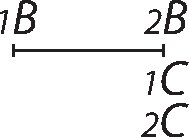
\includegraphics[width=0.11\textwidth]{%
gesamttex/edit_VIII,3/images/LH_37_05_060-061_d_060v.pdf%
}}
\quad
\lbrack\textit{Fig.~1}\rbrack %
%
\newline
\vspace{0.2em}Or le choc\protect\index{Sachverzeichnis}{choc} estoit de 4 degrés de force, donc chacun en receuvra 2, et aussi deux de vistesse.
%
Et\textsuperscript{\lbrack a\rbrack} \textit{C} en receuvra 4 et \textit{B} ayant 2 en avant
sera en repos. Au lieu que l'auteur conclut le contraire d'une maniere estrangement embrouillée. Le
%
co\lbrack roll\rbrack aire\textsuperscript{\lbrack b\rbrack} est veritabl\textlangle e\textrangle\ mais il ne se sauve point ainsi. 
%
\newline\vspace{-0.5em}
\newline%Marginalienapparat:
{\footnotesize \textsuperscript{\lbrack a\rbrack} Et\ \textit{ (1) }
\textbar\ \textit{B} \textit{ streicht Hrsg.} \textbar\ ayant 2 en receuvra 1 en \textbar\ arriere \textit{ streicht Hrsg.} \textbar\ \textit{ (2) } \textit{C} en receuvra 4 \textit{ (a) } \textbar\ et \textit{B} \textit{ streicht Hrsg.} \textbar\   \textit{ (b) } et \textit{B} ayant 2 en avant \textit{L}
\quad \textsuperscript{\lbrack b\rbrack} coollraire \textit{ L ändert Hrsg.}\vspace{-4mm}}%
}}%
%
(\protect\vphantom)+ Il y a bien à}{\lemma{separe}\Bfootnote{\textit{(1)} . (\protect\vphantom)+ Il y a bien à \textit{(2)} (\protect\vphantom)+ d'où il s'ensort que \textit{B} et \textit{C} iront ensemble vers l'occident ou du costé où \textit{B} alloit auparavant avec 2 degrés de vitesse +\protect\vphantom() \textit{(3)} . (\protect\vphantom)+ Il y a bien à \textit{L}}}
%
dire à cette
%
\edtext{demonstration. Sa}{\lemma{demonstration.}\Bfootnote{\textit{(1)}~ Il ne rend point de \textit{(2)} Sa \textit{L}}} 
%
supposition 3.\ de la manière qu'il l'explique dans la demonstration n'est pas bien seure, 
%
que deux corps s'approchans avec une vistesse respective,\protect\index{Sachverzeichnis}{vistesse respective} la moitié de cette 
%
\edtext{vistesse se}{%
\lemma{vistesse}%
\Bfootnote{%
\textit{(1)} soit %
\textit{(2)} se %
\textit{L}%
}}
%
doit attribuer à chacun, comme une vistesse reelle,\protect\index{Sachverzeichnis}{vistesse reelle} qu'il a. Pourqouy cela\,\lbrack\!?\rbrack
%%%
\pend
%
\pstart
Mais accordons cela, 
%
sans nous soucier si elle est reélle ou non; au moins on ne luy accordera pas la supposition 6.\ 
%
que deux corps même sans ressort\protect\index{Sachverzeichnis}{corps sans ressort} se reflechissent par le choc;\protect\index{Sachverzeichnis}{choc} et encor moins 
%
qu'\edtext{\lbrack ils se\rbrack}{%
\lemma{}%
\Bfootnote{%
elles %
\textit{L ändert Hrsg.}%
}}
%
reflechissent 
%
par des forces
%
\edtext{egales; puisque}{\lemma{egales;}\Bfootnote{\textit{(1)}~pourquoy \textit{(2)} puisque \textit{L}}} 
%
il les fait concourir non pas avec des forces egales\protect\index{Sachverzeichnis}{forces egales} mais avec des vistesses egales,
%
\edtext{pourquoy les fait}{\lemma{pourquoy}\Bfootnote{\textit{(1)} fait il \textit{(2)} les \textit{(a)} flait \textit{(b)} fait \textit{L}}} 
%
il reflechir
%
\edtext{autrement non avec}{\lemma{autrement}\Bfootnote{\textit{(1)}~avec \textit{(2)} non avec \textit{L}}} 
%
des vistesse mais avec des forces egales. C'est prendre des suppositions qui accommodent sans se soucier si elles sont fondées en
%
\edtext{raison. \edlabel{37_05_060-061_13a}Et quoyque}{\lemma{raison.}\Bfootnote{\textit{(1)} Il de \textit{(2)} Et quoyque \textit{L}}} 
%
la 7\textsuperscript{me} supposition soit raisonnable en elle même, que la reflexion\protect\index{Sachverzeichnis}{reflexion} se fait successivement\lbrack,\rbrack\ 
%
il luy donne pourtant un sens ou
%
\edtext{application extraordinaire. Il conçoit}{\lemma{application}\Bfootnote{\textit{(1)} estrange. Il \textbar\ s'imagine \textit{streicht Hrsg.} \textbar\  \textit{(2)} extraordinaire. Il conçoit \textit{L}}} 
%
que la force\protect\index{Sachverzeichnis}{force} commence à se
%
\edtext{reflechir lorsque}{\lemma{reflechir}\Bfootnote{\textit{(1)} avant que les deux corps concourans \textit{(2)} lorsque \textit{L}}} 
%
les deux corps concourans continuent encor à
%
\edtext{s'approcher. On n'accorde la}{\lemma{s'approcher}\Bfootnote{\textit{(1)} , ce qu'on n'accordera pas, \textit{(2)} . On n'accorde~\textit{L}}} 
%
7\textsuperscript{me} supposition que dans les corps à ressort,\protect\index{Sachverzeichnis}{corps à ressort} 
%
les quels se pressant continuellement jusqu'à ce que leur 
%
vistesse respective\protect\index{Sachverzeichnis}{vistesse respective} soit consumée, se restituent alors peu à
%
\edtext{peu; et commencent}{\lemma{peu;}\Bfootnote{\textit{(1)} mais ils ne se restituent point, peu \textit{(2)} et commencent à \textit{(a)} se \textit{(b)} aller \textit{L}}} 
%
en sens contraire. Mais on les fait 
%
\edtext{point aller en deux sens, ou}{\lemma{point}\Bfootnote{\textit{(1)}~se \textit{(2)}~aller
\textit{(a)} l'un con \textit{(b)} en deux sens,
\textit{(aa)} en mêm \textit{(bb)} ou \textit{L}}}
%
s'approcher et s'eloigner en même temps.%
\edlabel{37_05_060-061_13b}
\lbrack+\protect\vphantom()\rbrack
\pend
%
%
\vspace{0.5em} 
\pstart
\noindent
\foreignlanguage{ngerman}{\lbrack\textit{1.\ Auszug zur \glqq Seconde Loy\grqq}:\rbrack}
\pend
%
\pstart 
%
\edtext{\textit{\textso{Seconde Loy}. Si un corps sans ressort\protect\index{Sachverzeichnis}{corps sans ressort} paroist} 	%C-Fn
%
\edtext{\lbrack \textit{se}\rbrack}{%
\lemma{}%
\Bfootnote{%
ce %
\textit{L ändert Hrsg.\ nach Vorlage}%
}}
%
\textit{mouvoir seul vers un autre sans ressort\protect\index{Sachverzeichnis}{corps sans ressort} qui paroisse en repos}\lbrack,\rbrack\
%
\textit{la vistesse des deux ensemble après le choc\protect\index{Sachverzeichnis}{choc} sera le quotient de la force apparente\protect\index{Sachverzeichnis}{force apparente} de ce corps divisé par la somme des}
%
\edtext{\textit{masses. Soyent \textit{B}}}{\lemma{\textit{masses}.}\Bfootnote{ \textit{(1)} Soit \textit{B} en \textit{(2)} \textit{Soyent \textit{B}} \textit{L}}} 
%
\textit{et \textit{C} egaux et sans}
%
%
\edlabel{37_05_060-061_11a}%
\edtext{}{% 
{\xxref%
{37_05_060-061_11a}{37_05_060-061_11b}}%
\lemma{\textit{ressort}}%
\Bfootnote{%
\textit{(1)} \textit{B} viste %
\textit{(2)} \textit{B} masse %
\textit{L}%
}}%
\textit{ressort}\protect\index{Sachverzeichnis}{ressort}\lbrack,\rbrack}{\lemma{\textit{\textso{Seconde}} \lbrack...\rbrack\ \textit{ressort}}\Cfootnote{\cite{00526}a.a.O., S.~213.\hspace{25mm}}}
%
\textit{B} masse\edlabel{37_05_060-061_11b}
%
1.\ vistesse 4, \textit{C} masse 1.\ vistesse 0. Donc \textit{B} aura vistesse reelle 2, et \textit{C}
%
\edtext{aussi et leur}{\lemma{aussi}\Bfootnote{\textit{(1)}~. Or cela vient \textit{(2)} et leur \textit{L}}} 
%
percussion\protect\index{Sachverzeichnis}{percussion} cessera
%
\edtext{dès que deux degrés de force}{\lemma{dès que}\Bfootnote{\textit{(1)}~chacun \textit{(2)}~deux degrés de \textit{(a)}~vistesse \textit{(b)}~force \textit{L}}} 
%
seront reflechis, c'est à dire un de vistesse pour chacun. Ainsi chacun aura un degré en orient, et un en occident, et se
%
\edtext{repose. Mais pour faire}{\lemma{repose}\Bfootnote{\textit{(1)} , mais il y a deux degrés communs vers l'occident \textit{(2)} . Mais pour \textit{(a)}~leur donner \textit{(b)} faire \textit{L}}} 
%
avoir à \textit{B} et à \textit{C} 2 degrés egaux, j'ay supposé comme s'ils estoient avec moy 
%
dans le bateau,\protect\index{Sachverzeichnis}{bateau} allant de deux degrés en occident. Donc ce mouvement commun\protect\index{Sachverzeichnis}{mouvement commun} leur restera que
%
\edtext{\textit{si \textit{B} et \textit{C} se mettent en} 
%
\edtext{\textit{ressort parfait }}{%
\lemma{\textit{ressort}}%
\Bfootnote{%
\textit{(1)} dont %
\textit{(2)} \textit{parfait} %
\textit{L}%
}}%
%
dont \textit{la force egale}
%
\edtext{\lbrack \textit{à}\rbrack}{%
\lemma{}%
\Bfootnote{%
\textit{à} %
\textit{erg.\ Hrsg.\ nach Vorlage}%
}}
%
\textit{leur choc},%
}{\lemma{\textit{si \textit{B}} \lbrack...\rbrack\ \textit{choc}}\Cfootnote{\cite{00526}a.a.O., S.~213f.}} 
%
d \lbrack\textit{Text bricht ab.}\rbrack%
\edlabel{37_05_060-061_12b}\
%
\lbrack61~r\textsuperscript{o}\rbrack
\pend
%
%
\vspace{0.5em} 
\pstart
\noindent
\foreignlanguage{ngerman}{\lbrack\textit{2.\ Auszug zur \glqq Seconde Loy\grqq}:\rbrack}
\pend
%
\pstart 
%
\edtext{\textit{\textso{Seconde Loy}: 
%
Si un corps sans ressort\protect\index{Sachverzeichnis}{corps sans ressort} paroist se mouvoir seul 
%
vers un autre sans ressort,\protect\index{Sachverzeichnis}{corps sans ressort} qui paroisse en repos, 
%
la vistesse des deux ensemble après le choc\protect\index{Sachverzeichnis}{choc} sera le quotient de la 
%
force apparente\protect\index{Sachverzeichnis}{force apparente} de ce corps divisée par la somme des masses}}{\lemma{\textit{\textso{Seconde}} \lbrack...\rbrack\ \textit{masses}}\Cfootnote{\cite{00526}a.a.O., S.~213.}}. 
%
(\protect\vphantom)+ Comme sa demonstration me paroist fort embrouillée j'ay voulu la copier
%
\edtext{entiere: \lbrack+\protect\vphantom()\rbrack}{\lemma{entiere:}\Bfootnote{\textbar\ Soyent \textit{B} et \textit{C} deux corps égaux et sans ressort, et q \textit{gestr.} \textbar\ \textit{L}}}
%
\pend
%
\vspace{0.5em} 
\pstart
\noindent
\foreignlanguage{ngerman}{\lbrack\textit{3.\ Auszug zur \glqq Seconde Loy\grqq\ (A)}:\rbrack}
\pend
%
%
\pstart\centering
\hspace{1mm}\hspace{-1mm}% Trick, weil \edlabel nicht zu \par-Beginn sein darf
\edlabel{37_05_060-061_07a}%
\edtext{}{{\xxref{37_05_060-061_07a}{37_05_060-061_07b}}\lemma{\textit{\textso{Seconde}} \lbrack...\rbrack\ \textit{raisonnemens}}\Cfootnote{\cite{00526}a.a.O., S.~213f.}}%
\textit{Seconde Loi}.
\pend
%
\pstart\noindent
%
\textit{Si un corps sans ressort\protect\index{Sachverzeichnis}{corps sans ressort} paroit se mouvoir seul vers un autre sans ressort\protect\index{Sachverzeichnis}{corps sans ressort} qui paroisse en repos, la vitesse des deux ensemble après}
%
\edtext{\textit{l}\lbrack\textit{e}\rbrack}{\lemma{}\Bfootnote{la \textit{A ändert Hrsg. nach Vorlage}}} 
%
\textit{choc sera}
%
\edtext{\textit{l}\lbrack\textit{e}\rbrack}{\lemma{}\Bfootnote{la \textit{A ändert Hrsg. nach Vorlage}}} 
%
\textit{quotient de la force aparente\protect\index{Sachverzeichnis}{force apparente} de ce corps divisée par la somme des masses}. 
\pend
\newpage
\pstart
\textit{Soient \textit{B} et \textit{C} deux corps égaux et sans ressort,\protect\index{Sachverzeichnis}{corps égaux et sans ressort} et que \textit{B} vienne choquer \textit{C}
%
avec quatre degrez aparens de vitesse vers l'occident par la suposition 3\textsuperscript{e}.
%
\textit{B} n'aura que deux degrez reels vers \textit{C} et \textit{C} deux vers \textit{B}, qui me seront
%
communs avec lui, et que je transfererai à \textit{B}, de mesme qu j'ay}
%
\edtext{\textit{co}\lbrack\textit{u}\rbrack\textit{tume}}{\lemma{}\Bfootnote{contume \textit{A ändert Hrsg.\ nach Vorlage}}} 
%
\textit{de transferer aux rives de la mer}
%
\edtext{\textit{un}\lbrack\textit{e}\rbrack}{\lemma{}\Bfootnote{un \textit{A ändert Hrsg.\ nach Vorlage}}} 
%
\textit{vîtesse qui m'apartient; lorsque je suis dans un vaisseau\protect\index{Sachverzeichnis}{vaisseau} qui s'eloigne ou s'aproche d'elles. 
%
De plus la percussion\protect\index{Sachverzeichnis}{percussion} de ces deux corps cessera dès qu'un degré de \textit{B} et un degré de \textit{C} 
%
se seront reflechis; car alors, comme on vient de voir, \textit{B} et \textit{C} auront chacun un degré 
%
vers l'orient et chacun un degre vers l'occident, leur degré commun vers l'orient, après le choc\protect\index{Sachverzeichnis}{choc} simpatisera
%
avec un de mes deux degrez vers l'orient, dont la direction n'a pas changé: d'autant qu'ils n'ont pas entré 
%
en concurrence. Mais leur degré commun vers l'occident antipatisera avec mon autre degré vers l'orient, 
%
que je leur transfererai. C'est}
%
\edtext{\textit{pou}\lbrack\textit{r}\rbrack\textit{quoi}}{\lemma{}\Bfootnote{pousquoi \textit{A ändert Hrsg. nach Vorlage}}} 
%
\textit{\textit{B} et \textit{C} devront me paroitre après le choc\protect\index{Sachverzeichnis}{choc} se mouvoir ensemble vers l'occident avec 
%
deux de vitesse, quotient de quatre de force, qui est la mesme que paroissoit avoir \textit{B} 
%
avant le choc,\protect\index{Sachverzeichnis}{choc} divisez par deux de masse}. 
%
\pend
%
\pstart \textit{Maintenant si \textit{B} et \textit{C} se metent}
%
\edtext{\lbrack\textit{en}\rbrack}{\lemma{}\Bfootnote{\textit{en} \textit{erg.\ Hrsg.\ nach Vorlage}}} 
%
\textit{ressort,\protect\index{Sachverzeichnis}{ressort} et que leur ressort soit parfait,\protect\index{Sachverzeichnis}{ressort parfait} c'est à dire, que la force de leur ressort soit egale à celle
%
de leur choc, et que} 
%
\textit{cete force\protect\index{Sachverzeichnis}{force} se partage egalement entr'eux, comme celle du choc; \textit{B} et \textit{C} se refléchiront encore 
%
par le ressort\protect\index{Sachverzeichnis}{ressort} avec chacun un degré, sçavoir chacun avec le degré direct que le choc lui avoit laissé}. 
%
\lbrack61~v\textsuperscript{o}\rbrack\ 
%
\textit{Les deux degrez de \textit{B} reflechis vers l'orient, simpatiseront avec mes deux degrez vers l'orient. 
%
C'est pourqoui \textit{B} me paroistra immobile; et ces deux degrez de \textit{C}}
%
\textit{refléchis vers l'occident, antipatiseront avec mes deux degrez vers l'orient, que je lui}
%
\edtext{\textit{trans}\lbrack\textit{f}\rbrack\textit{ererai}}{\lemma{}\Bfootnote{transererai \textit{A ändert Hrsg. nach Vorlage}}} 
%
\textit{encore. Partant \textit{C} se mouvra après le choc avec quatre degrez aparens vers l'occident.} %
\pend
%
\pstart
\textit{Dans les autres cas, comme dans ceux-ci les experiences favorisent mes raisonnemens}.\edlabel{37_05_060-061_07b} \pend
%
\vspace{0.5em} % evtl. entfernen
\pstart
\noindent
\lbrack\foreignlanguage{ngerman}{\textit{L}:}\rbrack
%
\pend
%
\pstart
\edtext{(\protect\vphantom)+}{% 
\lemma{(\protect\vphantom)+}% 
\Cfootnote{%
Die Klammer bleibt offen.%
}}
%
Tout cecy estant brouillé, voicy comment je comprend la chose 
%
conformement au sentiment de l'auteur: 
%
Soyent \textit{B} et \textit{C} egaux et sans ressort.\protect\index{Sachverzeichnis}{ressort} \textit{B} masse 1, vistesse 4, \textit{C} masse 1, vistesse 0,
%
vistesse respective\protect\index{Sachverzeichnis}{vistesse respective} 4, partagée egalement, sera 2 pour \textit{B}, et 2 pour \textit{C}, qui sera leur vistesse reelle\protect\index{Sachverzeichnis}{vistesse reelle} selon
%
\edtext{l'auteur. Et leur}{\lemma{l'auteur.}\Bfootnote{\textit{(1)} Or leur pe \textit{(2)} Et \textit{(a)} deu \textit{(b)} leur \textit{L}}}
%
percussion\protect\index{Sachverzeichnis}{percussion} 
%
\edtext{cessera, dès que}{\lemma{cessera,}\Bfootnote{\textit{(1)} deux \textit{(2)}~dès \textit{(a)} qu'on aura \textit{(b)} que \textit{L}}} 
%
2 degrés de force seront reflechis, c'est 
%
\edtext{à dire 1}{%
\lemma{ à dire}%
\Bfootnote{%
\textit{(1)} 2 de vi %
\textit{(2)} un %
\textit{(3)} 2 de %
\textit{(4)} 1 %
\textit{L}%
}}
%
de vistesse pour un chacun. Car
%
\edtext{les 2}{\lemma{les}\Bfootnote{\textit{(1)} 4 \textit{(2)} 2 \textit{L}}} 
%
qui
%
\edtext{restent des vistesses \lbrack qu'\rbrack ils}{\lemma{restent}\Bfootnote{\textit{(1)} de ceux qui \textit{(2)} des vistesses \textit{(a)} reelles \textit{(b)} \textbar\ qu' \textit{erg.\ Hrsg.} \textbar\ ils \textit{L}}} 
%
avoient, chacun 1, seront compensés, et chacun aura un degré en occident, et un en orient. 
%
Cependant pour faire avoir à \textit{B} la vistesse reélle\protect\index{Sachverzeichnis}{vistesse reelle} 2, et \textit{C} aussi, il a valu les concevoir 
%
dans un bateau,\protect\index{Sachverzeichnis}{bateau} allant d'orient en occident comme \textit{B},
%
\edtext{ave\lbrack c\rbrack}{\lemma{}\Bfootnote{ave \textit{L ändert Hrsg.}}} 
%
2 degrés de vistesse, ainsi cette vistesse leur restera après le choc, et ils iront ensemble en occident
%
 avec 2 degrés de vistesse. Mais de plus si nous leur donnons un parfait ressort,\protect\index{Sachverzeichnis}{ressort parfait} qui conserve la force du
%
\edtext{choc perdue, qui estoit}{\lemma{choc}\Bfootnote{\textit{(1)} , qui est de 2 degrés \textit{(2)} perdue, qui  \textit{(a)} chacun \textit{(b)} estoit \textit{L}}} 
%
de 4 degrés, chacun en aura deux, et \textit{B} ayant 2
%
\edtext{degré\lbrack s\rbrack}{\lemma{}\Bfootnote{degré \textit{L ändert Hrsg.}}} 
%
en occident
%
\edtext{auparavant, et 2 en}{%
\lemma{auparavant,}%
\Bfootnote{%
\textit{(1)} et \textbar\ en \textit{streicht Hrsg.}\ \textbar\ %
\textit{(2)} et 2 en %
\textit{L}%
}}
%
orient par la reflexion\protect\index{Sachverzeichnis}{reflexion} du ressort;\protect\index{Sachverzeichnis}{ressort} et \textit{C} en ayant 2 degrés en occident 
%
auparavant, et deux encor par la reflexion,\protect\index{Sachverzeichnis}{reflexion} \textit{B} sera en repos, et \textit{C} seul ira en occident 
%
avec 4 degres. Mais j'ay deja dit que je trouve à redire qu'il donne reflexion\protect\index{Sachverzeichnis}{reflexion} sans ressort.\protect\index{Sachverzeichnis}{ressort} %
\pend
%
\pstart
%
Essayons de comprendre son sentiment en general. \pend
%
\pstart Masse \textit{a}, vistesse \textit{v}, et masse \textit{b} vistesse \textit{x}\lbrack,\rbrack\
%
toutes deux prises comme du même
%
\edtext{costé. Vistesse d'appropinquation\protect\index{Sachverzeichnis}{vistesse d'appropinquation}}{\lemma{costé.}\Bfootnote{\textit{(1)} Celle du basteau \textit{(a)}$x:$ \textit {(b)} $v+x,:2$ \textit{(aa)}~celle \textit{(bb)} la vistesse reelle \textit{(2)} Vistesse d'appropinquation \textit{L}}} 
%
$v-x$, vistesse reelle d'\textit{a} est $v-x,:2$ et vistesse reelle de \textit{b} est $-v+x,:2$ 
%
celle du bateau\protect\index{Sachverzeichnis}{bateau} $v+x,:2$. 
%
Leur choc\protect\index{Sachverzeichnis}{choc} cessera\lbrack,\rbrack\
%
\edtext{\lbrack dès que\rbrack}{%
\lemma{}%
\Bfootnote{%
deux %
\textit{L ändert Hrsg.}%
}}
%
la force reflechie\protect\index{Sachverzeichnis}{force reflechie} sera
%
\edtext{$ff$, la moitie}{\lemma{$ff$,}\Bfootnote{\textit{(1)}~dont la \textit{(2)} la moitie \textit{L}}} 
%
à chacun sera $ff:2$ et la vistesse
%
\edtext{reflechie\protect\index{Sachverzeichnis}{vistesse reflechie}}{\lemma{}\Bfootnote{reflechie \textit{erg. L}}} 
%
de l'un sera $ff:2a$, de l'autre
%
\edtext{$ff:2\lbrack b$\rbrack,}{\lemma{}\Bfootnote{$ff:2a$ \textit{L ändert Hrsg.}}} 
%
j'eu
%
or la force\protect\index{Sachverzeichnis}{force} $ff$, soustraite des forces $\overline{v-x}\;a:2+\overline{v-x}\;b:2$, 
%
laissera $\overline{v-x}\;\overline{a+b}:2-ff$ dont la moitié sera $\overline{v-x}\cdot\overline{a+b}:4-ff:2$. 
%
Ce qui divisé par \textit{a} donnera $\overline{v-x}\cdot\overline{a+b}:4a-ff:2a$, et par \textit{b}, 
%
donnera $\overline{v-x}\cdot\overline{a+b}:4b-ff:2b$. Ostons du premier sa vistesse reflechie\protect\index{Sachverzeichnis}{vistesse reflechie} $ff:2a$,
%
\edtext{et du second}{\lemma{et}\Bfootnote{\textit{(1)} de l'au \textit{(2)} du second \textit{L}}} 
%
la vistesse reflechie\protect\index{Sachverzeichnis}{vistesse reflechie}
%
\edtext{$ff:2b$. Le premier fera}{\lemma{$ff:2b$.}\Bfootnote{\textit{(1)} Il faut qu' \textit{(2)} Le premier fera \textit{L}}} 
%
$\overline{v-x}\cdot\overline{a+b}:4a-ff:a$. Le second fera $\overline{v-x}\cdot\overline{a+b}:4b-ff:b$ 
%
et changeant le signe du dernier, pour les concevoir allans du même coste, 
%
il y aura $\overline{v-x}\;\overline{a+b}:4a-ff:a= ff:b\;\overline{-v+x}\;\overline{a+b}:4b$ 
%
\protect\rule[-4mm]{0mm}{10mm}et il y aura $\overline{v-x}\;\overline{a+b}\;\overline{\dfrac{1}{a}+\dfrac{1}{b}}:4=ff\overline{\dfrac{1}{a}+\dfrac{1}{b}}$, 
%
donc $ff=\overline{v-x}\;$%
%
\edtext{$\overline{a+b}:4$. Donc $ff$ estant}{\lemma{$\overline{a+b}:4$.}\Bfootnote{\textit{(1)} Mais je crois qu'il y a un erreur dans le calcul \textit{(a)} car \textit{(aa)} substi \textit{(bb)} soustrahant, \textit{(b)} donc soustrahant $ff:2a$ de \textit{(2)} Donc $ff$ estant \textit{L}}} 
%
trouvé, on voit quelle vistesse reste à chacun après la detraction de la reflexion,\protect\index{Sachverzeichnis}{reflexion} 
%
la perte doit estre jointe à celle du bateau.\protect\index{Sachverzeichnis}{bateau} Et puis à celle du
%
\edtext{ressort.\protect\index{Sachverzeichnis}{ressort} Il}{\lemma{ressort.}\Bfootnote{\textit{(1)} Mais il \textit{(2)} Il \textit{L}}} 
%
sera bon de l'achever pour voir s'il viendra tousjours ce que les autres voyes donnent. 
%
Il me semble que j'ay commis quelque erreur de calcul. Il vaudra resumer ce dernier calcul. \pend
\count\Bfootins=1200%
\count\Afootins=1200%
\count\Cfootins=1200 